\documentclass[a4paper,12pt]{article}
\usepackage[utf8]{inputenc}
\usepackage[english]{babel}
\usepackage{hyperref}
\usepackage{graphicx}
\usepackage{glossaries}
\usepackage{minted}
\usepackage{wrapfig}
\usepackage{float}
\usepackage{todonotes}
\begin{document}
	%Build: pandoc -s  .\Nextcloud.tex -o Nextcloud.md --toc --listings --verbose
	\title{Setup encrypted Nextcloud with reverse proxy}
	\author{Jan-Ruben Schmid}
	\maketitle
	\tableofcontents
	\pagebreak
	\section{Introduction}
	This guide describes how to setup a Nextcloud server from scratch on a SBC (Single board computer). Even my setup is based on Ubuntu 18 with a \href{https://rockpi.org/rockpi4}{RockPi4}, this tutorial will also describe the equivilative on a Raspberry Pi, since it is far more common.
	To follow this guide, no previous knowledge is required, but it will be helpful. \newline
	This tutorial will guide you from flashing your SBC until your Nextcloud server is ready to use, with an encrypted communication and accessible from everywhere in the world with a public URL.\newline
	The last section \ref{sec:SetupVsCode} describes my personal preferred SSH setup, which makes it easy to quickly access and maintain the devices. 
	\section{Required hardware}
	\begin{itemize}
		\item \href{https://rockpi.org/rockpi4}{RockPi4} or similar, for example Raspberry Pi 4
		\item Micro SD card (minimum size: 16GB, recommended: 32GB)
		\item External hard drive
		\item Wifi or LAN access
	\end{itemize}
	I recommend the RockPi4, Raspberry Pi 4 with 4GB Ram, or something similar.
	\section{Summary of the used tools}
	\subsection{What's a RockPi}
	The Rock Pi 4 is like a Raspberry Pi a Single Board Computer (SBC). The available interfaces are a Gigabit Ethernet, USB 3 interface, and a 2.4 GHz wifi module.
	\subsection{What's Nextcloud}
	Nextcloud started in 2016 as a Fork from Owncloud. Nextcloud is a free Software to store, share and save data at your own server. It is licensed  under the AGPLv3 license. Mobile clients are available for Linux, Mac-OS, Windows, as well as for IOS and Android.
	\subsection{What's Let's Encrypt}
	Let's Encrypt is a free, automated, and open certificate authority brought to you by the nonprofit Internet Security Research Group (ISRG) \href{https://letsencrypt.org/}{[letsencrypt]}.
	\subsection{What's MS Azure}
	Microsoft Azure is a cloud computing platform from Microsoft with the services such as SQL Azure or AppFabric, which is primarily aimed at software developers. Azure was announced in October 2008, and started with the code name "Project Red Dog". Since February 2010 the platform is officially available.
	
	\section{Setup SBC}
	To setup the SBC, a computer with a micro SD card slot is required. To remote access it, SSH has to be activated.
	\subsection{Flash SBC}
	Download \href{https://www.balena.io/etcher/}{balenaEtcher} to Flash your SBC.
	Download the Image for:
	\begin{itemize}
		\item Raspberry Pi
		\begin{itemize}
			\item \href{https://www.raspberrypi.org/software/operating-systems/}{Raspberry Pi OS Lite}
		\end{itemize}
		\item RockPi 
		\begin{itemize}
			\item \href{https://wiki.radxa.com/Rockpi4/downloads}{Ubuntu Server 20.04}
		\end{itemize}
	\end{itemize}
	After the download succeeded, open Balena Etcher, select the Image and double-check your selected device, see the image below. Be careful, all data will be deleted on the device.
	\begin{figure}[H]
		\centering
		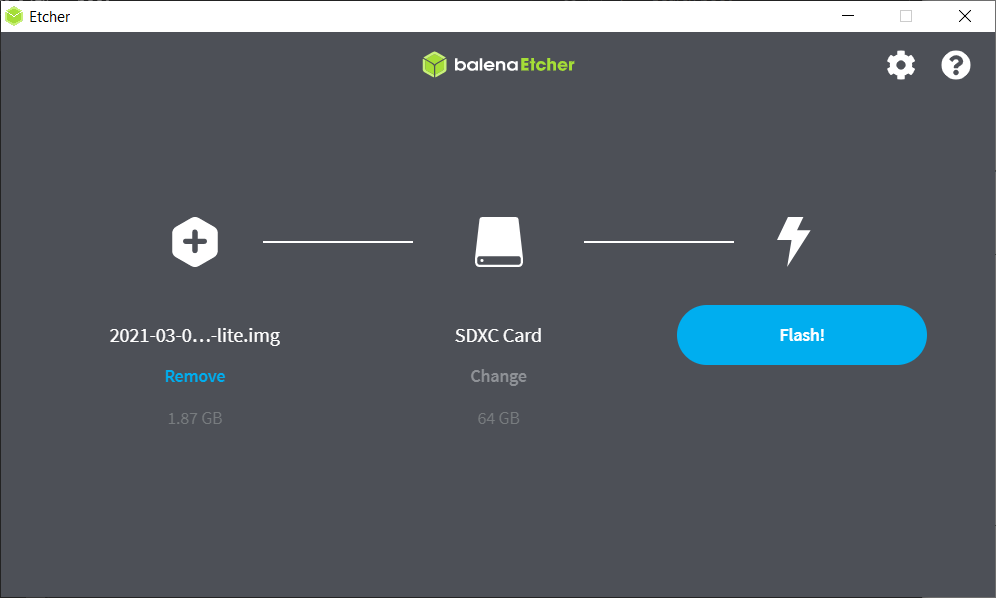
\includegraphics{images/BalenaEtcherFlash.png}
		\caption{Balena flash SD card}
	\end{figure}
	\subsection{Enable SSH}
	Since 2016, SSH has to be activated manually. This is done by creating a file with the name "ssh" in the boot partition of your flashed SD card.
	\subsubsection{Linux}
	Open a terminal, change to the boot partition directory, which is most likely in "/media/yourUserName/".
	Create a new file by entering the command:
	\begin{minted}{sh}
		touch ssh
	\end{minted}
	\subsubsection{Windows}
	Open the drive "boot" and create a new file with the name "ssh", without the file extension ".txt". If the boot partition is not mounted, try to unplug and plug your SD card. If you can't see the file unselect "Hide extensions for known file types", see the figure below. 
	\begin{figure}[H]
		\centering
		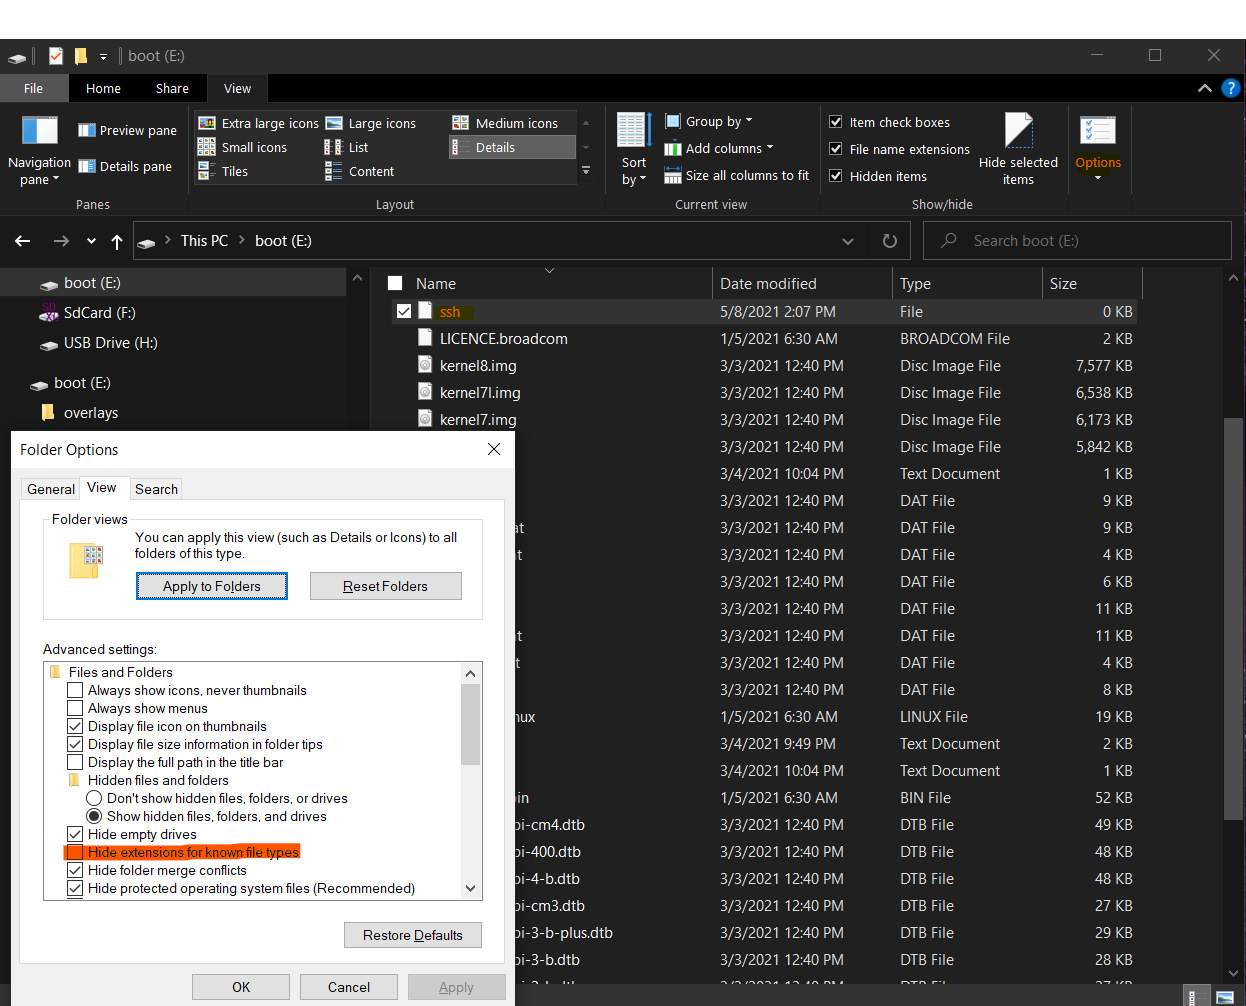
\includegraphics[width=0.7\linewidth]{images/WindowsAddSSHFile.png}
		\caption{Add file ".ssh" in boot partition}
		\label{fig:WindowsAddSSHFile}
	\end{figure}
	\subsection{SSH}
	Connect your SBC to the same network as your PC.
	An easy way to get the local address of your SBC, is by an arp scan. This can be done in Linux and Windows by the command:
	\begin{minted}{sh}
		arp -a
	\end{minted}
	To determine your device after the arp scan, compare it with the physical address range of the  \href{https://udger.com/resources/mac-address-vendor-detail?name=raspberry_pi_foundation}{Raspberry Pi} or \href{https://udger.com/resources/mac-address-vendor-detail?name=realtek_semiconductor_corp}{RockPi}.
	To establish a connection to your SBC, open a terminal and enter:
	\begin{itemize}
		\item Raspberry:
		\begin{itemize}
			\item ssh pi@yourLocalIpAddress, password: \textbf{raspberry}
		\end{itemize}
		\item RockPi4: 
		\begin{itemize}
			\item ssh rock@yourLocalIpAddress, password: \textbf{rock}
		\end{itemize}
	\end{itemize}
	Change your password with:
	\begin{minted}{sh}
		sudo passwd
	\end{minted}
	\subsubsection{Recommended: setup ssh key}
	See section\ref{sec:SetupSShKeys}
\todo{are we gonna do this here?}
	\section{Setup proxy}
	This section describes how to setup a reverse proxy with Ms Azure. This step is only required if you can't forward a port (no access to router or if you have a DS-lite connection). If this is not the case for you, skip this section and have a look \href{https://help.dyn.com/remote-access/getting-started-with-remote-access/}{here}.\newline
	 The basic setup is described in following figure:
	\begin{figure}[H]
		\centering
		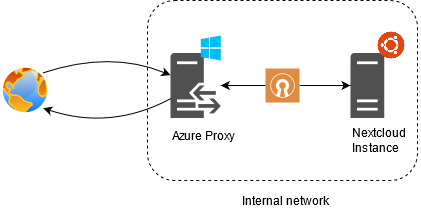
\includegraphics{images/ProjectOverviewOvpn.png}
	\end{figure}
	Because the virtual machine of Ms Azure has a static port, this port can be used to access our SBC. The SBC establishes a connection to Ms Azure with OpenVPN (or alternatively WireGuard), and the traffic is redirected.
	The costs are ~5\$ per month. Azure offers a free student account credit.
	\subsection{Create Ms Azure account}
	Create a \href{https://azure.microsoft.com/en-us/free/}{free account} or \href{https://azure.microsoft.com/en-au/free/students/}{free student account}.
	Afterwards, sign in to the \href{https://portal.azure.com}{azure portal}. 
	\begin{itemize}
		\item 	Press "Create a resource"
		\item Service: Select latest Ubuntu server version -> Create
		\item Tab: "Create a virtual machine - Basic" 
		\begin{itemize}
			\item Virtual machine name: Reverse proxy for Nextcloud
			\item Region: Your home region
			\item Size: smallest size, currently: Standard\_B1ls - 1 vcpu, 0.5 GiB memory
			\item Authentication type: SSH public key
			\item Select inbound ports: Select SSH(22), HTTPS, HTTP
			\item press "next"
		\end{itemize}
		\item Tab: "Create a virtual machine - Disk" 
		\begin{itemize}
			\item OS disk type: Standard HDD
			\item Advanced: Use managed disks -> unselect (you pay only for the storage you are using)
		\end{itemize}
		\item Review +create -> Create
		\item Press "Download private key and create resource"
		\item Copy the downloaded key to your .ssh folder
		\begin{itemize}
			\item Linux: \textasciitilde/.ssh
			\item Windows: C:/Users/UserName/.ssh
		\end{itemize}
	\end{itemize}
	Go back to "All resources" -> Virtual machine -> Networking -> Inbound port rules -> Add inbound port rules
	Set the settings as shown in the figure:
	\begin{figure}[H]
		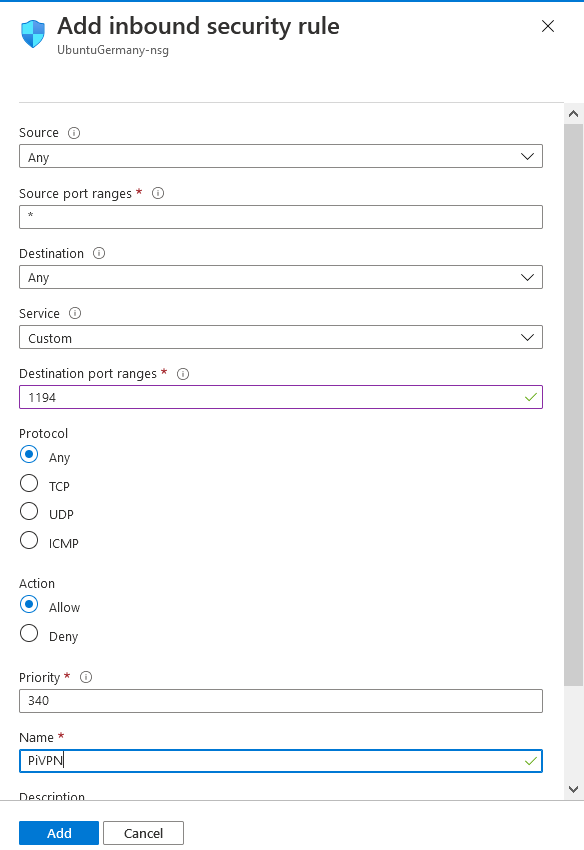
\includegraphics{images/PiVPNInboundRule.png}
	\end{figure}
	\section{Setup a dynamic dns}
	To access your Nextcloud with a web address instead of an IP address, create a free account at a dynamic dns provider, for example \href{https://my.noip.com/#!/dynamic-dns}{noip}. Select a host name and domain and set the IP address from your Azure server. Since Azure provides a static IP address, no further steps are required.
	\begin{figure}
		\includegraphics{images/NoIpSetHostname}
	\end{figure}
	\section{Setup OpenVPN}
	\subsection{Server}
	Before you continue, I recommend to follow section \ref{sec:SetupSShKeys} and \ref{sec:SetupVsCode}, until "RaspberryPiOverAzure". \newline
	Open a SSH connection with Vs Code to AzureUbuntu. Open on the left panel of Vs Code the remote explorer, right click "AzureUbuntu" and select "Connect in current window".
	If no new Terminal opens, select "Terminal-> New Terminal". \newline
	Congratulations, you have now a connection to your Ms Azure server.\newline
	Before we start, you should update the system, enter following in your Vs Code terminal:
	\begin{minted}{sh}
		sudo apt update && sudo apt upgrade -y
	\end{minted}
	Let's install OpenVPN, where \href{https://www.pivpn.io/}{PiVPN} is an easy way to set it up. It works for Raspbian and Ubuntu.
	Enter following in your Vs Code terminal:
	\begin{minted}{sh}
		 curl -L https://install.pivpn.io | {sh} 
	\end{minted}
	Follow the installation instructions. You can navigate with "Tab". Select your choice with "Space". Choose OpenVPN as VPN.  Use your previously created DNS entry. 
	\subsubsection{Create client profile}
	Connect with Vs Code to Azure. 
	\begin{minted}{sh}
		pivpn -a -nopass
	\end{minted}
	Press the folder icon in Vs Code -> open folder -> open "/home/azureuser/ovpns".
	Right click on your ovpn profile and download it to your development machine.
	\subsection{Client}
	Install the OpenVPN client on your SBC:
	\begin{minted}{sh}
		sudo apt install openvpn
	\end{minted}
	Change the file type of your OpenVPN profile to .conf.
	Open the folder "/etc/openvpn" with Vs Code and paste your OpenVPN profile. It will now automatically connect to Azure after a reboot. Restart the service to establish a connection:
	\begin{minted}{sh}
		sudo systemctl restart openvpn
	\end{minted}
	Now you can setup the SSH access to your raspberry through Azure with a proxy, see section \ref{sec:SetupVsCode}.
	\section{Setup Nextcloud}
	Everything is now prepared to get started. First, we will setup Nextcloud on the SBC, afterwards some configurations at the reverse proxy are required.
	Most of the following information are from the latest \href{https://docs.nextcloud.com/server/latest/admin_manual/installation/source_installation.html}{Nextcloud installation instructions}.
	The required dependencies get installed with:
	\begin{minted}{sh}
	echo "deb http://mirrordirector.raspbian.org/raspbian/ buster main contrib non-freee rpi">/etc/apt/sources.list.d/10-buster.list
	sudo apt update
	sudo apt install git nano unzip nginx postgresql curl libcurl4 redis-server php7.3-fpm php7.3-curl php7.3-gd php7.3-intl php7.3-bcmath php7.3-gmp php7.3-imagick imagemagick php7.3-mbstring php7.3-opcache php7.3-xml php7.3-xmlrpc php7.3-zip php7.3-apcu php7.3-common php7.3-intl php-pear php7.3-apcu php7.3-xml php7.3-mbstring php7.3-zip  php7.3-pgsql php7.3-intl php-imagick php7.3-json php7.3-bz2 php-smbclient redis-server php-redis -y
	\end{minted}
	Set your default php version to 7.3:
	\begin{minted}{sh}
		sudo update-alternatives --set php /usr/bin/php7.3
	\end{minted}
	Install Nextcloud:
	\begin{minted}{sh}
		cd /var/www/
		wget https://download.nextcloud.com/server/releases/latest.zip
		sudo unzip latest.zip
		sudo rm latest.zip
		sudo rm -R html
		sudo mv nextcloud html
		sudo chown -R www-data:www-data /var/www/html
	\end{minted}
	\subsection{Change mount location of the hard drive}
	To automount your HDD at each boot , get the UUID of your device with:
	\begin{minted}{bash}
		sudo blkid
	\end{minted}
	It should look similar to:
	\begin{figure}
		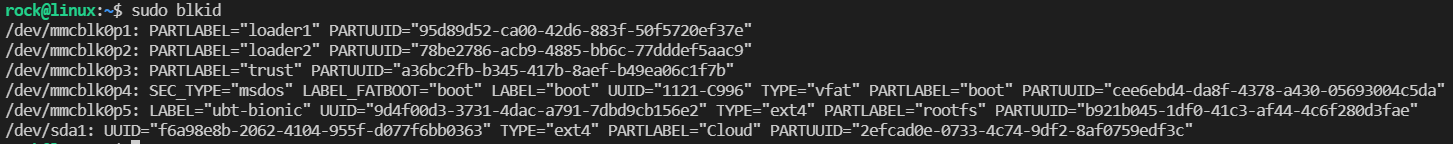
\includegraphics{images/BlkId.png}
	\end{figure}
	Adjust your fstab
	\begin{minted}{bash}
		sudo nano /etc/fstab
	\end{minted}
	It should look similar to:
	\begin{figure}
		\includegraphics{images/fstab.png}
	\end{figure}
	In case you run into issues, have a look \href{https://www.linuxbabe.com/desktop-linux/how-to-automount-file-systems-on-linux}{here}.
	\subsection{Configure nginx}
	Open /etc/nginx/sites-enabled/default
	\begin{minted}{nginx}
		upstream php-handler {
			server unix:/var/run/php/php7.3-fpm.sock;
		}
		server {
			set $myDomain myDomain;
			listen 80;
			listen [::]:80;
			add_header Strict-Transport-Security "max-age=15768000; includeSubDomains; preload;";
			add_header X-Content-Type-Options nosniff;
			add_header X-XSS-Protection "1; mode=block";
			add_header X-Robots-Tag none;
			add_header X-Download-Options noopen;
			add_header X-Permitted-Cross-Domain-Policies none;
			add_header X-Frame-Options "SAMEORIGIN";
			add_header Referrer-Policy "no-referrer" always;
			
			# Remove X-Powered-By, which is an information leak
			fastcgi_hide_header X-Powered-By;
			# Path to the root of your installation
			root /var/www/html/;
			
			location = /robots.txt {
				allow all;
				log_not_found off;
				access_log off;
			}
			
			# set max upload size
			client_max_body_size 5120M;
			client_body_buffer_size 4096k;
			fastcgi_buffers 64 4K;
			
			# Enable gzip but do not remove ETag headers
			gzip off;
			gzip_vary on;
			gzip_comp_level 4;
			gzip_min_length 256;
			gzip_proxied expired no-cache no-store private no_last_modified no_etag auth;
			gzip_types application/atom+xml application/javascript application/json application/ld+json application/manifest+json application/rss+xml application/vnd.geo+json application/vnd.ms-fontobject application/x-font-ttf application/x-web-app-manifest+json application/xhtml+xml application/xml font/opentype image/bmp image/svg+xml image/x-icon text/cache-manifest text/css text/plain text/vcard text/vnd.rim.location.xloc text/vtt text/x-component text/x-cross-domain-policy;
			
			location / {
				rewrite ^ /index.php;
			}
			
			location ~ ^/(?:build|tests|config|lib|3rdparty|templates|data)/ {
				deny all;
			}
			location ~ ^/(?:\.|autotest|occ|issue|indie|db_|console) {
				deny all;
			}
			
			location ~ ^\/(?:index|remote|public|cron|core\/ajax\/update|status|ocs\/v[12]|updater\/.+|oc[ms]-provider\/.+)\.php(?:$|\/)  {
				fastcgi_split_path_info ^(.+\.php)(/.*)$;
				try_files $fastcgi_script_name =404;
				include fastcgi_params;
				fastcgi_param SCRIPT_FILENAME $document_root$fastcgi_script_name;
				fastcgi_param PATH_INFO $fastcgi_path_info;
				fastcgi_param modHeadersAvailable true;
				fastcgi_param front_controller_active true;
				fastcgi_pass php-handler;
				fastcgi_intercept_errors on;
				fastcgi_request_buffering off;
			}
			
			
			location ~ ^\/(?:updater|oc[ms]-provider)(?:$|\/) {
				try_files $uri/ =404;
				index index.php;
			}
			
			location ~ \.(?:css|js|woff2|svg|gif)$ {
				try_files $uri /index.php$uri$is_args$args;
				add_header Cache-Control "public, max-age=15778463";
				add_header X-Content-Type-Options nosniff;
				add_header X-XSS-Protection "1; mode=block";
				add_header X-Robots-Tag none;
				add_header X-Download-Options noopen;
				add_header X-Permitted-Cross-Domain-Policies none;
				# Optional: Don't log access to assets
				access_log off;
			}
			
			
			
			location ~ \.(?:png|html|ttf|ico|jpg|jpeg)$ {
				try_files $uri /index.php$uri$is_args$args;
				# Optional: Don't log access to other assets
				access_log off;
			}
		}
	\end{minted}
	Replace "myDomain" with your domain. It should be similar to "myNextCloud.spdns.eu".
	Now restart nginx with:
	\begin{minted}{sh}
		sudo systemctl restart nginx
	\end{minted}
	\subsubsection{Setup PostgreSQL user and database}
	\begin{minted}{sh}
		sudo -u postgres psql
		\password postgres
		\q
		#Enter save password for user
		sudo -u postgres createuser -P -d nextcloud
		sudo -u postgres createdb -O nextcloud nextcloud
	\end{minted}
	\subsubsection{Setup Nextcloud}
	Type the URL from your SBC in your browser.
	\textbf{Don't use your administrator user name or password as login data}. Choose a save password, since the website will be accessible through the web later.
	Set as User and Database nextcloud. The password for your database is the previously defined postgresql password.
	\begin{figure}
		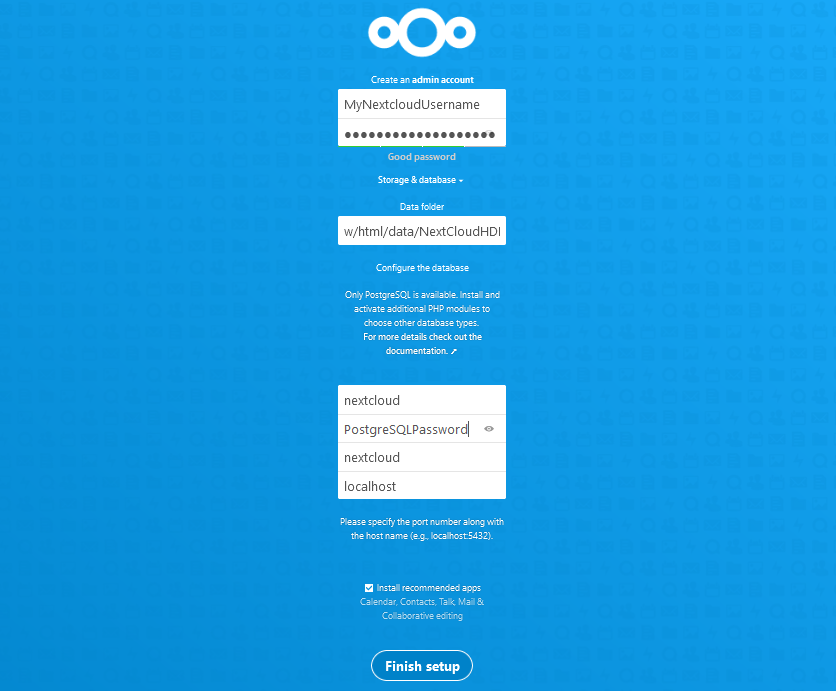
\includegraphics{images/NextcloudSetup}
	\end{figure}
	\paragraph{Setup Memory Cache}
	Nextcloud recommends using the memcache. Set it up by:
	\begin{minted}{sh}
		sudo nano /var/www/html/config/config.php
	\end{minted}
	Append following line:
	\begin{minted}{sh}
		'memcache.local' => '\OC\Memcache\APCu',
	\end{minted}
	\paragraph{Configure environemnt variables, use OPcache}
	\begin{minted}{sh}
		sudo nano /etc/php/7.3/fpm/pool.d/www.conf
	\end{minted}
	Search with nano "Ctrl+w" for \textit{;env[HOSTNAME]} and uncomment it by removing the semicolon in front of the line:
	\begin{minted}{sh}
		;env[HOSTNAME] = $HOSTNAME
		;env[PATH] = /usr/local/bin:/usr/bin:/bin
		;env[TMP] = /tmp
		;env[TMPDIR] = /tmp
		;env[TEMP] = /tmp
	\end{minted}
	Save the file with "Ctrl+x"\newline
	Open
	\begin{minted}{sh}
		sudo nano /etc/php/7.3/fpm/php.ini
	\end{minted}
	replace 
	\begin{minted}{sh}
		memory_limit = 16G
	\end{minted}
	and append
	\begin{minted}{sh}
		opcache.enable=1
		opcache.enable_cli=1
		opcache.interned_strings_buffer=8
		opcache.max_accelerated_files=10000
		opcache.memory_consumption=128
		opcache.save_comments=1
		opcache.revalidate_freq=1
	\end{minted}
	Save the file with "Ctrl+x".
	\paragraph{Use system cron service for background jobs}
	It is recommended to execute the background jobs with cron. For that we will configure a systemd service and systemd timer
	\begin{minted}{sh}
		sudo nano /etc/systemd/system/nextcloudcron.service
	\end{minted}
	Add
	\begin{minted}{sh}
		[Unit]
		Description=Nextcloud cron.php job
		
		[Service]
		User=www-data
		ExecStart=/usr/bin/php -f /var/www/html/cron.php
		
		[Install]
		WantedBy=basic.target
	\end{minted}
	Save the file with "Ctrl+O \& Ctrl+X"
	\begin{minted}{sh}
		sudo nano /etc/systemd/system/nextcloudcron.timer
	\end{minted}
	Add 
	\begin{minted}{sh}
		[Unit]
		Description=Run Nextcloud cron.php every 15 minutes
		
		[Timer]
		OnBootSec=5min
		OnUnitActiveSec=15min
		Unit=nextcloudcron.service
		
		[Install]
		WantedBy=timers.target
	\end{minted}
	Start and enable service with
	\begin{minted}{sh}
		sudo systemctl start nextcloudcron.timer
		sudo systemctl enable nextcloudcron.timer
	\end{minted}
		
	restart nginx
	\begin{minted}{sh}
		sudo systemctl restart nginx
	\end{minted}
	\section{Setup reverse proxy}
	Install nginx and certbot
	\begin{minted}{sh}
		sudo apt install python3 nginx certbot python3-certbot-nginx
	\end{minted}
	Get a certificate
	\begin{minted}{sh}
		sudo certbot --nginx
	\end{minted}
	Follow the setup, enter your domain if requested. \newline
	Configure your reverse proxy, determine the local IP address of your SBC with:
	\begin{minted}{sh}
		pivpn -c
	\end{minted}
	Keep in mind that your SBC has to be connected to the VPN server to get and IP address, remember the Virtual IP, we will need it later.\newline
	Configure your reverse proxy:
	
	\begin{minted}{sh}
		sudo nano /etc/nginx/sites-enabled/default
	\end{minted}
	Your configuration should look similar like following, replace the 	proxy\_pass with your Virtual IP. Append the \.well-known locations as well.
	\begin{minted}{nginx}
		server {
			listen 80 default_server;
			listen [::]:80 default_server;
		}
		
		server {
			root /var/www/html;
			
			# Add index.php to the list if you are using PHP
			#index index.html index.htm index.nginx-debian.html;
			server_name yourDomain.spdns.eu; # managed by Certbot
			
			location / {
				# First attempt to serve request as file, then
				# as directory, then fall back to displaying a 404.
				#try_files $uri $uri/ =404;
				proxy_headers_hash_max_size 512;
				proxy_headers_hash_bucket_size 64;
				proxy_set_header Host $host;
				proxy_set_header X-Forwarded-Proto $scheme;
				proxy_set_header X-Real-IP $remote_addr;
				proxy_set_header X-Forwarded-For $proxy_add_x_forwarded_for;
				
				add_header Front-End-Https on;
				proxy_pass http://10.8.0.1/; #Replace with the Virtual Ip of the SBC
			}
			location /.well-known/{
				rewrite ^/\.well-known/carddav https://$server_name/remote.php/dav/;
				rewrite ^/\.well-known/caldav https://$server_name/remote.php/dav/;
				rewrite ^/\.well-known/webfinger https://$server_name/index.php/.well-known/webfinger;
				rewrite ^/\.well-known/nodeinfo https://$server_name/index.php/.well-known/nodeinfo;
			}
			
			
			listen 443 ssl; # managed by Certbot
			ssl_certificate /etc/letsencrypt/live/yourDomain.spdns.eu/fullchain.pem; # managed by Certbot
			ssl_certificate_key /etc/letsencrypt/live/yourDomain.spdns.eu/privkey.pem; # managed by Certbot
			include /etc/letsencrypt/options-ssl-nginx.conf; # managed by Certbot
			ssl_dhparam /etc/letsencrypt/ssl-dhparams.pem; # managed by Certbot
			
		}
		
		server {
			if ($host = yourDomain.spdns.eu) {
				return 301 https://$host$request_uri;
			} # managed by Certbot
			
			
			listen 80 ;
			listen [::]:80 ;
			server_name yourDomain.spdns.eu;
			return 404; # managed by Certbot
		}
		
		server {
			if ($host = yourDomain.spdns.eu) {
				return 301 https://$host$request_uri;
			} # managed by Certbot
			
			
			server_name yourDomain.spdns.eu;
			listen 80;
			return 404; # managed by Certbot
		}
	\end{minted}
	Change the max body size of nginx
	\begin{minted}{sh}
		sudo nano /etc/nginx/nginx.conf
	\end{minted}
	set client\_max\_body\_size = 128G;"
	\section{Recommended development environment}
	This section is optional, but in my opinion it's worth spending some minutes to setup the remote access on your local machine.
	\subsection{Setup SSH Keys}\label{sec:SetupSShKeys}
	This section describes how connect to your raspberry pi without a password promt.\newline
	Open a terminal on your development machine
	\begin{minted}{sh}
		cd ~/.ssh
		ssh-keygen
		#FileName promt: SSHForMyRaspi
		# Press enter until key is generated, for ease of use don't setup a password
		#Now, let's copy your key to the raspberry
		scp .\SSHForMyRaspi.pub pi@myLocalIpAddress:/.ssh/authorized_keys
	\end{minted}
	It's important that the key get copied to the file "authorized\_keys", if not it will not work.
	\subsection{Setup and install Vs Code}\label{sec:SetupVsCode}
	\begin{itemize}
		\item Windows
		\begin{itemize}
				\item Download VsCode for \href{https://code.visualstudio.com/}{Windows}
		\end{itemize}
		\item Linux
		\begin{itemize}
			\item  Install VsCode for Linux: \newline
			\begin{minted}{sh}
sudo snap install --classic code
			\end{minted}
		
		\end{itemize}
		\item Install the \href{https://marketplace.visualstudio.com/items?itemName=ms-vscode-remote.vscode-remote-extensionpack}{Remote extension}
	\end{itemize}
	\subsection{Direct connection to device}
	\begin{itemize}
		\item Open Vs Code and select the "Remote explorer" on the left
		\item Press on the configure button next to SSH Targets, select "../yourUserName/.ssh/config"
	\end{itemize}
	\begin{minted}{sh}
		IdentityFile ~/.ssh/SSHForMyRaspi
		Host AzureUbuntu
			HostName IpAddressOfAzure
			IdentityFile C:/Users/yourUserName/.ssh/YourDownloadedAzureKey.pem
			User azureuser
		Host Raspberry
			HostName RaspberryPiLocalIp
			User pi
	\end{minted}
	Let's have a look what's happening here:
	\begin{itemize}
		\item IdentityFile
		\begin{itemize}
			\item Your private key which is required to connect to your SBC, you got in in the section \ref{sec:SetupSShKeys}
		\end{itemize}
		\item AzureUbuntu
		\begin{itemize}
			\item This is your Azure reverse proxy. You can get the public IP from your azure portal
			\item The file YourDownloadedAzureKey is the azure access key, you got that after you created the virtual machine.
		\end{itemize}
		\item Raspberry
		\begin{itemize}
			\item This is your local address of the Raspberry, you can access it when you are in your local network
		\end{itemize}
	\end{itemize}
	\subsection{Connection via proxy}
	This allows you to connect to your SBC outside from the local network
	\begin{itemize}
		\item Open Vs Code and select the "Remote explorer" on the left
		\item Press on the configure button next to SSH Targets, select "../yourUserName/.ssh/config"
	\end{itemize}
	Append to the previous configured file
	\begin{minted}{sh}
		Host RaspberryOverAzure
			HostName YourRaspberryOpenVpnIpInAzure
			User pi
			ProxyCommand C:\Windows\System32\OpenSSH\ssh.exe -q -W %h:%p AzureUbuntu
	\end{minted}
	Let's have a look again whats happening here
	\begin{itemize}
		\item A connection to AzureUbuntu is established
		\item From Azure, a connection to your Raspberry is established
		\item "AzureUbuntu" from the proxycommand has to match the Host name of Azure
	\end{itemize}
\end{document}